\section{Mobile Application Architecture}
\label{sec:mobile-application-architecture}

The Stockrium mobile application is implemented with React Native, Expo, TypeScript, and Expo Router. Its architecture follows a layered, screen-oriented structure in which every route represents a user-visible task and reusable components encapsulate market cards, charts, forms, bottom sheets, and financial sections. The client is intentionally responsible for interaction, presentation, lightweight input validation, and local preferences. Authentication decisions, authoritative financial data, technical calculations, and AI execution remain behind the backend API.

The application combines Expo Router's file-based stack navigation with a custom five-tab interface. File-based routes manage transitions between major screens, while the main application shell uses a pager to support horizontal tab movement and preserve the distinctive central Chatbot control. This hybrid navigation model provides conventional stack behavior for detailed tasks without restricting the visual and interaction design of the primary tabs.

\subsection{Layered Mobile Architecture}
\label{subsec:layered-mobile-architecture}

Figure~\ref{fig:stockrium-mobile-architecture} presents the mobile client as a layered architecture. The layers separate application-wide composition, user-facing presentation, state ownership, API access, and persistent device storage. The arrows represent the principal dependencies and data exchanges rather than a strict invocation sequence.

\begin{figure}[H]
    \centering
    \IfFileExists{figures/chapter4/stockrium_mobile_architecture.png}{%
        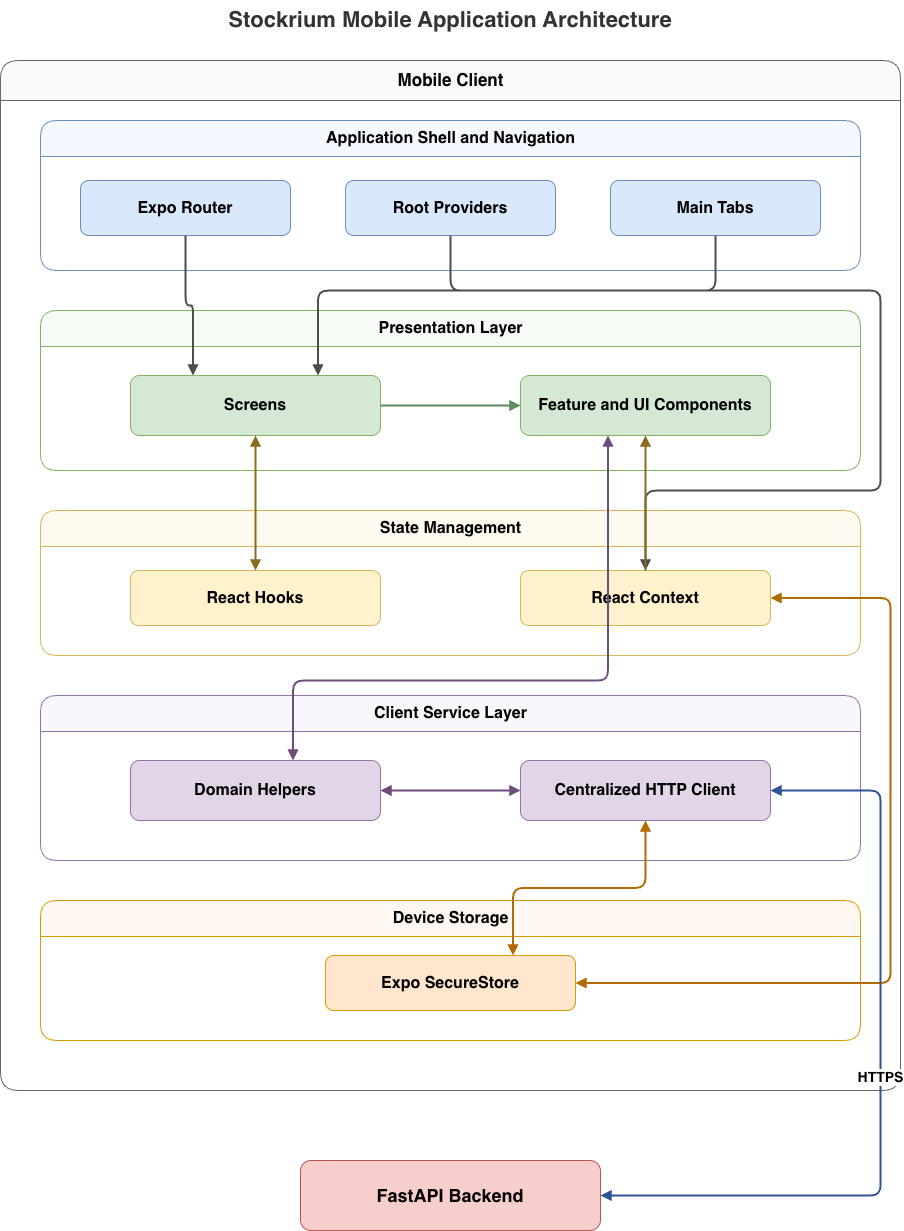
\includegraphics[width=0.72\textwidth,height=0.82\textheight,keepaspectratio]{figures/chapter4/stockrium_mobile_architecture.png}%
    }{%
        \fbox{\parbox[c][6.0cm][c]{0.88\textwidth}{\centering
        Expected architecture diagram:\\
        \texttt{figures/chapter4/stockrium\_mobile\_architecture.png}}}%
    }
    \caption{Layered architecture of the Stockrium mobile application}
    \label{fig:stockrium-mobile-architecture}
\end{figure}

The application shell and navigation layer establishes the client-wide execution environment. Expo Router maps files to stack destinations, the root providers supply safe-area, gesture, localization, and theme facilities, and the custom main tabs coordinate the five primary application areas. This layer determines which screen is active and ensures that shared infrastructure is available before feature content is rendered.

The presentation layer contains route-level screens and reusable feature and UI components. Screens coordinate a user task, receive route parameters, and compose the required feature components. Reusable components encapsulate domain-specific sections and common interface elements so that market data, stock details, authentication controls, news content, and analysis results can be presented consistently without duplicating implementation across routes.

State is kept close to the scope in which it is needed. React Hooks manage transient screen or component state, including loading indicators, selections, form values, and fetched results. React Context distributes the smaller set of cross-cutting presentation preferences, particularly theme and language. Values that must survive application restarts, such as session tokens and selected local preferences, are stored through Expo SecureStore instead of remaining only in memory.

The client service layer separates UI code from transport details. Feature-oriented domain helpers translate screen operations into typed application requests and delegate them to the centralized HTTP client. The HTTP client constructs HTTPS requests to the FastAPI backend, attaches stored credentials, coordinates token refresh, and returns parsed responses to the calling helper. It also exchanges session data with SecureStore, while providers restore persisted preferences into React Context. This separation allows screens and components to focus on interaction and presentation, while authentication recovery, endpoint construction, and secure persistence remain centralized.

\subsection{Navigation Structure}
\label{subsec:mobile-navigation-structure}

The root layout establishes the providers and infrastructure that every screen requires. It first loads the Roboto font family and then nests the application inside a safe-area provider, gesture-handler root, localization provider, and theme provider. An Expo Router stack manages screen transitions with the default header disabled because Stockrium screens provide their own headers. A global session-expired modal is rendered beside the stack so that authentication failure can be communicated regardless of which screen is currently active.

The index route acts as a navigation gateway rather than a visible home screen. It reads the persistent onboarding flag and the stored session. If onboarding has not been completed, the user is redirected to the Onboarding route. If onboarding is complete, both token values are present, and the refresh token has not expired, the user is redirected to the main Tabs route. Otherwise, the Authentication route is opened. The gateway does not require the access token itself to remain valid because an expired access token can be renewed transparently by the centralized HTTP client.

The authentication branch contains two related paths. The account-creation path proceeds from the sign-up form to one-time password (OTP) verification. Successful verification confirms the email address and returns the user to authentication; it does not create an authenticated session automatically. The account-recovery path proceeds from email input to OTP verification and then to the new-password screen before returning to authentication. Returning users can sign in with application credentials or Google and move directly to the Tabs route. Navigation replacement is used after onboarding or successful authentication so that the Android back action does not return the user to a completed entry screen.

The main shell contains Overview, Market, Chatbot, News, and Profile. It is implemented with a pager and a custom bottom bar rather than Expo Router's default tab navigator. A tab is mounted only after it has been visited, reducing the initial work required to construct data-heavy market and news screens. The active-tab indicator is animated, and the Chatbot is represented by a raised central button instead of a conventional tab item. Swiping the pager or selecting a bottom-bar item updates the same active index.

Figure~\ref{fig:mobile-navigation-structure} summarizes the principal route relationships. It groups routes according to user goals rather than listing every modal bottom sheet as an independent destination.

\begin{figure}[H]
    \centering
    \IfFileExists{figures/chapter4/stockrium_mobile_navigation_structure.png}{%
        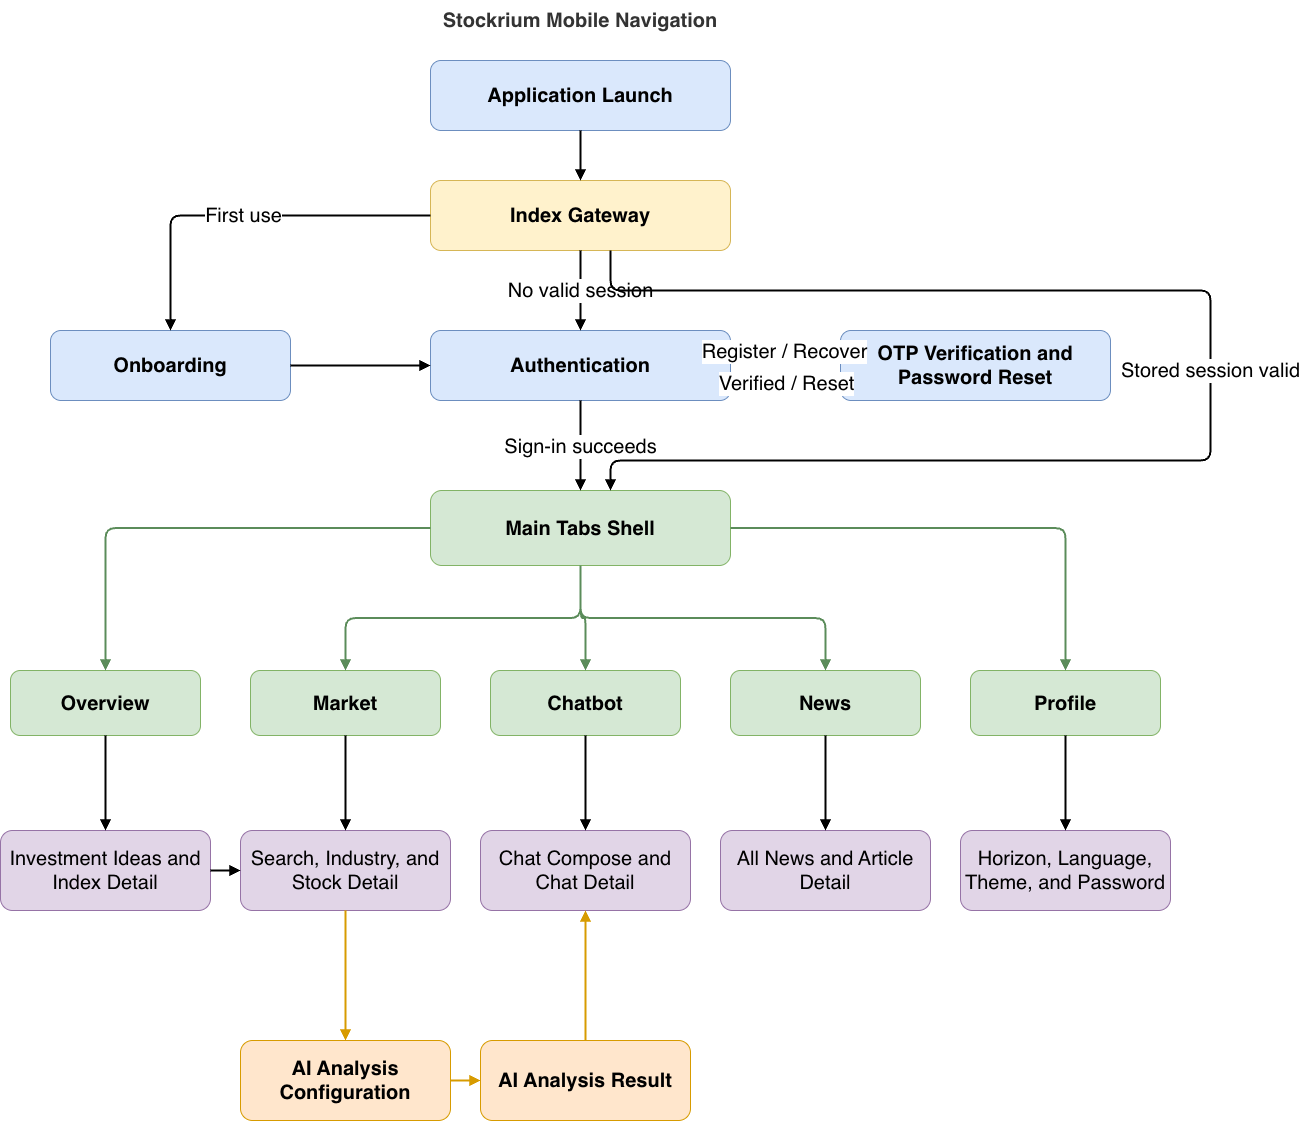
\includegraphics[width=0.96\textwidth,height=0.82\textheight,keepaspectratio]{figures/chapter4/stockrium_mobile_navigation_structure.png}%
    }{%
        \fbox{\parbox[c][5.5cm][c]{0.92\textwidth}{\centering
        Export the Draw.io diagram as\\
        \texttt{figures/chapter4/stockrium\_mobile\_navigation\_structure.png}}}%
    }
    \caption{Principal navigation structure of the Stockrium mobile application}
    \label{fig:mobile-navigation-structure}
\end{figure}

The Stock Detail route is a particularly important navigation hub. It can be opened from search results, watchlist entries, investment-idea lists, industry visualizations, market highlights, and related-stock cards. It receives the stock symbol as a route parameter and passes the same symbol to its child sections. A floating AI button opens the configuration route with that symbol, after which the result route receives the analysis mode and serialized manual selection. This parameterized navigation keeps the user focused on one company across data inspection and AI analysis.

News and chatbot routes follow a similar pattern. General or categorized lists open a shared article-detail route using article parameters. The Chatbot tab displays available sessions; composing or selecting a session opens Chat Detail with a session identifier. An AI result can create and seed a new session before navigating to that same Chat Detail route, allowing ordinary conversations and analysis follow-ups to reuse one interface.

\subsection{API Integration and Client State}
\label{subsec:api-integration-client-state}

The mobile application does not call \texttt{fetch} directly from every screen. Feature-specific helpers expose typed functions such as market-index retrieval, stock-price retrieval, company-profile retrieval, watchlist operations, investment-horizon persistence, analysis execution, and chat-session management. These helpers build endpoint paths and request bodies, then delegate network behavior to a single HTTP function. This structure keeps route strings, response interpretation, and authentication recovery out of visual components.

\subsubsection{Base URL and Request Construction}

The API base URL depends on the build environment. Production builds use the deployed Railway backend. During development, iOS uses the local host, Android or a physical Expo device derives the development machine address from the Metro host when possible, and the Android-emulator fallback uses its host mapping. Centralizing this decision prevents screens from embedding environment-specific addresses.

For each request, the shared client reads the access and refresh tokens from SecureStore. It constructs JSON headers and adds the bearer access token when present. The feature helper then receives the parsed Stockrium response and converts its error code and data into a compact success/failure shape appropriate for the calling screen.

\subsubsection{Automatic Token Refresh}

An HTTP 401 Unauthorized response triggers coordinated token renewal. If no refresh is currently running, the failed request becomes the refresh leader and submits the stored refresh token to the authentication endpoint. Other requests that receive 401 during this interval subscribe to the same operation instead of issuing additional refresh calls. If renewal succeeds, a new access token is saved and the subscribed requests retry using the new value, followed by the original leader request. Figure~\ref{fig:mobile-token-refresh-flow} illustrates this sequence.

\begin{figure}[H]
    \centering
    \resizebox{0.86\textwidth}{!}{%
    \begin{tikzpicture}[
        box/.style={draw, rounded corners=5pt, fill=blue!7, minimum width=3.0cm, minimum height=1.0cm, align=center, font=\small},
        decision/.style={draw, rounded corners=10pt, fill=yellow!15, minimum width=2.8cm, minimum height=1.0cm, align=center, font=\small},
        action/.style={draw, rounded corners=5pt, fill=green!9, minimum width=3.2cm, minimum height=1.0cm, align=center, font=\small},
        failure/.style={draw, rounded corners=5pt, fill=red!8, minimum width=3.2cm, minimum height=1.0cm, align=center, font=\small},
        flow/.style={-{Latex[length=2.2mm]}, line width=0.65pt, gray!80},
        guard/.style={font=\scriptsize, text=black}
    ]
        \node[box] (screen) at (0,0) {Screen calls a\\feature helper};
        \node[box] (session) at (0,-1.8) {Read session and\\send bearer request};
        \node[decision] (status) at (0,-3.6) {Response\\status};
        \node[action] (success) at (5.0,-3.6) {Return parsed response\\to the screen};
        \node[decision] (active) at (0,-5.5) {Refresh already\\in progress?};
        \node[action] (wait) at (-3.7,-7.5) {Subscribe and wait for\\the shared new token};
        \node[action] (refresh) at (3.7,-7.5) {Call refresh endpoint\\with refresh token};
        \node[decision] (refreshstatus) at (3.7,-9.4) {Refresh\\succeeds?};
        \node[action] (retry) at (0,-11.4) {Save token, notify\\subscribers, and retry};
        \node[failure] (expired) at (7.4,-11.4) {Emit session-expired\\event and show modal};

        \draw[flow] (screen.south) -- (session.north);
        \draw[flow] (session.south) -- (status.north);
        \draw[flow] (status.east) -- node[above, guard] {not 401} (success.west);
        \draw[flow] (status.south) -- node[right, guard] {401} (active.north);
        \draw[flow] (active.south west) -- node[above left, guard] {yes} (wait.north east);
        \draw[flow] (active.south east) -- node[above right, guard] {no} (refresh.north west);
        \draw[flow] (refresh.south) -- (refreshstatus.north);
        \draw[flow] (refreshstatus.south west) -- node[above left, guard] {yes} (retry.north east);
        \draw[flow] (refreshstatus.south east) -- node[above right, guard] {no} (expired.north west);
        \draw[flow] (wait.south) |- node[left, guard] {on success} (retry.west);
    \end{tikzpicture}%
    }
    \caption{Coordinated access-token refresh in the mobile HTTP client}
    \label{fig:mobile-token-refresh-flow}
\end{figure}

If refresh fails or returns incomplete token data, the client emits a global authentication-expired event. The modal registered in the root layout becomes visible, removes local session data after confirmation, and replaces the current route with Authentication. This event-based mechanism avoids passing an expiration callback through every component.

\subsubsection{State Scope and Persistence}

Stockrium uses local React state for screen-specific data, React context for a small number of application-wide preferences, SecureStore for persistent device state, and backend storage for user-owned domain state. A large global state framework is not required because market and detail screens can request their own independent data and because user-specific records such as watchlist entries and conversations already have authoritative server representations.

\begin{table}[H]
    \centering
    \caption{Client-state scopes in the Stockrium mobile application}
    \label{tab:client-state-scopes}
    \small
    \begin{tabularx}{\textwidth}{>{\raggedright\arraybackslash}p{3.1cm} >{\raggedright\arraybackslash}p{4.1cm} X}
        \toprule
        \textbf{State scope} & \textbf{Mechanism} & \textbf{Examples} \\
        \midrule
        Screen-local transient state & React state, refs, memoization, effects, and a keyboard-visibility hook & Loading flags, fetched lists, chart type, selected time frame, active indicator, keyboard visibility, bottom-sheet visibility, search text, selected radar axis, and form validation. \\
        \addlinespace
        Cross-screen presentation state & React Context & Current light/dark theme, selected language, and translated text lookup. \\
        \addlinespace
        Persistent device state & Expo SecureStore & Access token, refresh token, onboarding completion, theme, language, and the saved AI-analysis preset. \\
        \addlinespace
        Navigation state & Expo Router and the custom PagerView & Current stack route, route parameters, active main tab, and the set of tabs that have been visited and mounted. \\
        \addlinespace
        Global transient events & Event emitters & Authentication expiration and programmatic switching of the custom tab shell. \\
        \addlinespace
        Authoritative user data & Backend API and Supabase & Watchlist symbols, search history, investment horizon, account profile, chat sessions, and chat messages. \\
        \bottomrule
    \end{tabularx}
\end{table}

The Theme and Localization providers load their stored values before rendering children. This prevents a visible flash in which the application initially renders with the wrong theme or language. Theme changes and language selection are immediately reflected through context and persisted for the next launch. The AI configuration uses the same hydration principle: its saved mode, source toggles, indicator groups, and weights are read before subsequent changes are written, preventing the default state from overwriting an existing preset during initialization.

The manual analysis screen also maintains consistency among related controls. Submission is enabled only when at least one evidence source remains usable; an enabled technical or fundamental source must contain at least one selected subcategory; and changing enabled sources redistributes weights among the active choices. These client checks improve the request before submission, while the backend schema remains responsible for authoritative validation.

Overall, the mobile design keeps screen composition, visualization, session recovery, and user preferences close to the client while delegating business rules and authoritative data to backend services. File-based routes make task transitions explicit, domain components reduce duplication, and the shared HTTP layer gives every screen consistent authentication behavior. The next section describes the server-side architecture that receives these client requests.
